
\subsection{Blog in Django}
\begin{frame}{Blog in Django}
\begin{block}{My Blog}
I made an application called My Blog in the report. It consists of all the necessary modules as the other blogs does have.
The different moduled are:
\begin{itemize}
\item My Posts: It displays all the posts done by me.
\item My Poems: The poems posted by me are displayed here.
\item My Images/ Sketches: It contains all the images and sketches posted.
\end{itemize}
I have synchronized Mysql database with it thus all the values of posts, Poems and Images are fetched directly from database.
\end{block}
\end{frame}
\newpage
\subsection{My Blog's front page}
\begin{frame}{Front page of blog}
\begin{figure}[h]
\centering 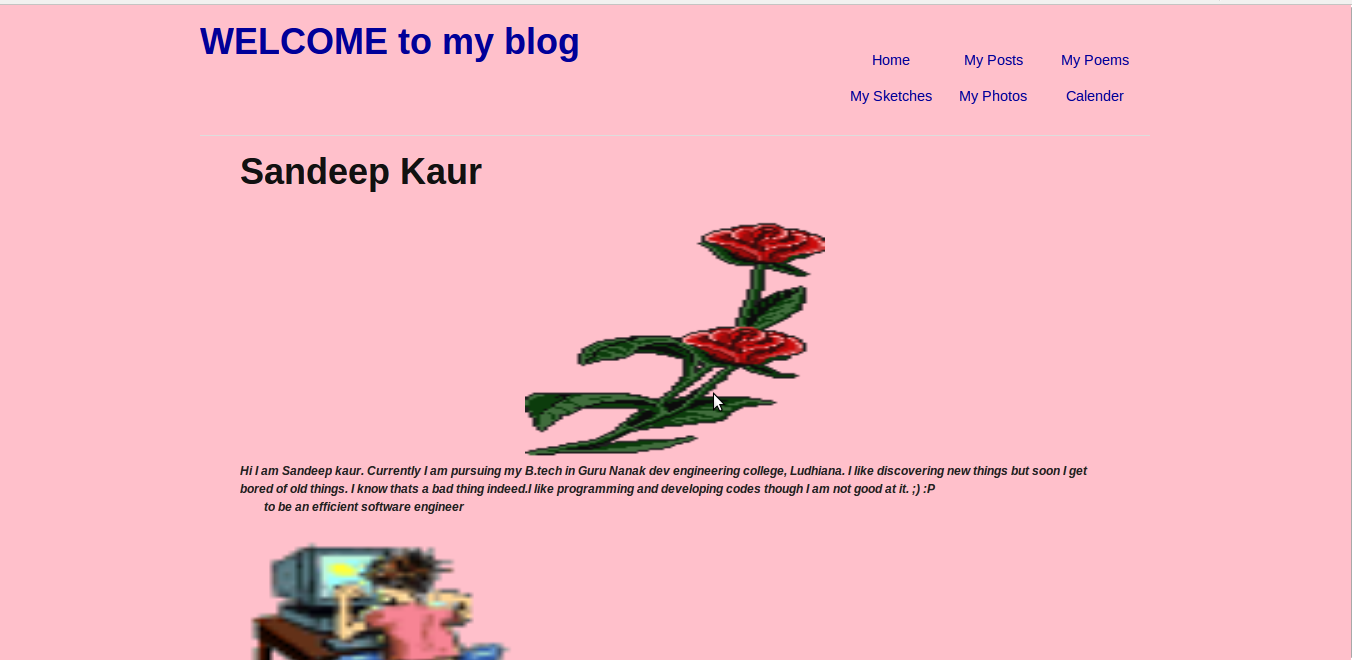
\includegraphics[scale=0.2]{bg.png}
\caption{Index page of Blog}
\end{figure}
\end{frame}

